\chapter{Evaluation}\label{chap:evaluation}

This chapter presents the findings and results from the experiments outlined in the specification and design chapter (\ref{chap:specification-design}) as well as the implementation chapter (\ref{chap:implementation}). We evaluate the classifiers' performance, first on their respective datasets and then on a different dataset to assess transferability. Additionally, we explore the SHAP (SHapley Additive exPlanations) values for each experiment to reason about the importance of features in the models.

\section{Performance Evaluation}\label{sec:performance-evaluation}

As described in section (\ref{sec:TransferabilityEvaluation}), the classifiers are evaluated on their respective datasets and subsequently on another dataset to assess transferability. The performance metrics assessed include accuracy, precision, recall, and F1 score, as outlined in Chapter~\ref{chap:specification-design}, Section~\ref{subsec:EvaluationMetrics}. Results are illustrated in Figures~\ref{fig:classifier_performance_same_dataset} and~\ref{fig:classifier_performance_across_dataset}.

\subsection{Performance on the Same Dataset}\label{subsec:performance-same-dataset}

\begin{figure}[H]
\centering
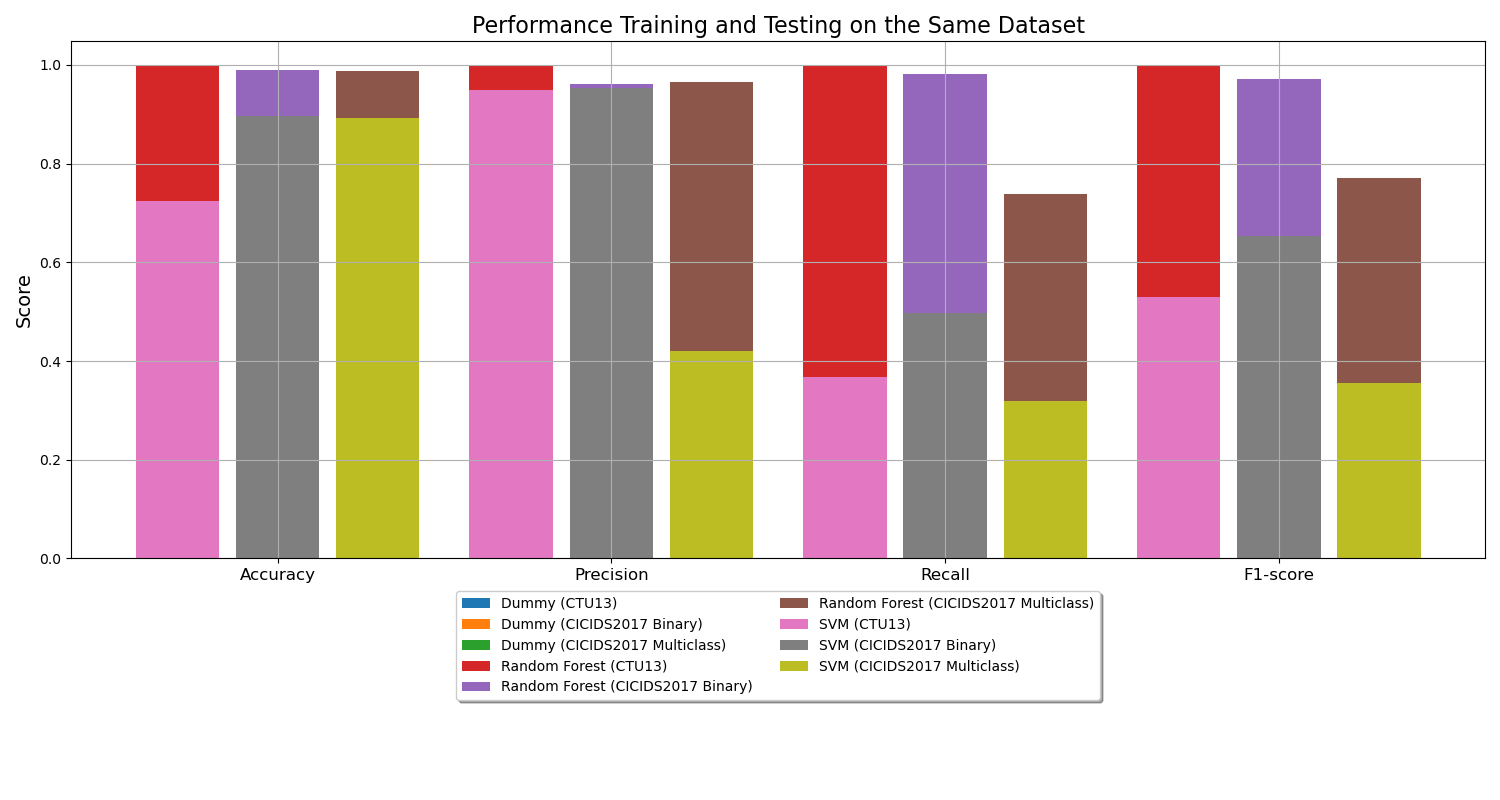
\includegraphics[width=\textwidth]{img/Classifier_Performance_Same_Dataset.png}
\caption{Classifiers' performance on the same datasets.}\label{fig:classifier_performance_same_dataset}
\end{figure}

When testing the classifiers’ performance on the datasets they were trained on, we observed promising results. The Random Forest model achieved high performance across all metrics on both the CTU13 and CICIDS2017 datasets for binary classification. It recorded an accuracy, precision, recall, and F1 score of 0.99 on CTU13, with comparable scores on CICIDS2017 (accuracy=0.99, precision=0.96, recall=0.98, F1=0.97). These results suggest that the Random Forest classifiers effectively learned patterns to distinguish between benign and malicious traffic, aligning with prior studies on their efficacy in network attack detection, as discussed in Chapter~\ref{chap:relevant-work}, Section~\ref{sec:RandomForestIntrusion}.

For multi-class classification on CICIDS2017, the Random Forest model performed respectably, achieving an F1 score of 0.78 (accuracy=0.99, precision=0.90, recall=0.76). Although there is scope for improvement to achieve deployment-ready performance, the model demonstrated clear learning compared to a dummy classifier baseline of 0.66. Overall, Random Forest classifiers consistently outperformed dummy baselines on their training datasets, underscoring their ability to identify discriminative patterns, as noted in Chapter~\ref{chap:background}, Section~\ref{sec:classifiers}.

In contrast, the SVM classifiers underperformed relative to both Random Forest models and dummy classifiers when evaluated on their training datasets. The binary SVM on CTU13 achieved an accuracy of 0.73, precision of 0.96, recall of 0.37, and F1 score of 0.53. Similar results were observed on CICIDS2017 (accuracy=0.73, precision=0.96, recall=0.37, F1=0.65). The multi-class SVM on CICIDS2017 recorded an accuracy of 0.89 but exhibited low precision (0.42), recall (0.32), and F1 score (0.35). These findings indicate that the current SVM implementations struggled to learn distinguishing patterns, even on their training datasets, contrasting with prior studies highlighting SVM effectiveness in network intrusion detection, as discussed in Chapter~\ref{chap:relevant-work}, Section~\ref{sec:SVMIntrusion}. Improvements are likely required, as explored in Chapter~\ref{chap:conclusion-future-work}.

\subsection{Feature Importance Analysis on Same Dataset}\label{subsec:feature-importance-analysis-same-dataset}

To gain insight into how Random Forest models make predictions, we analyse SHAP values. SHAP, an explainable AI technique, assigns importance scores to features for each prediction, elucidating the model’s decision-making process, as detailed in Chapter~\ref{chap:background}, Section~\ref{sec:explainable}. The appendix listing~\ref{chap:feature-list} provides guidance on interpreting the SHAP value graphs in this section.

\subsubsection{Random Forest Model on CTU13}\label{subsec:rf-ctu13}

\begin{figure}[H]
\centering
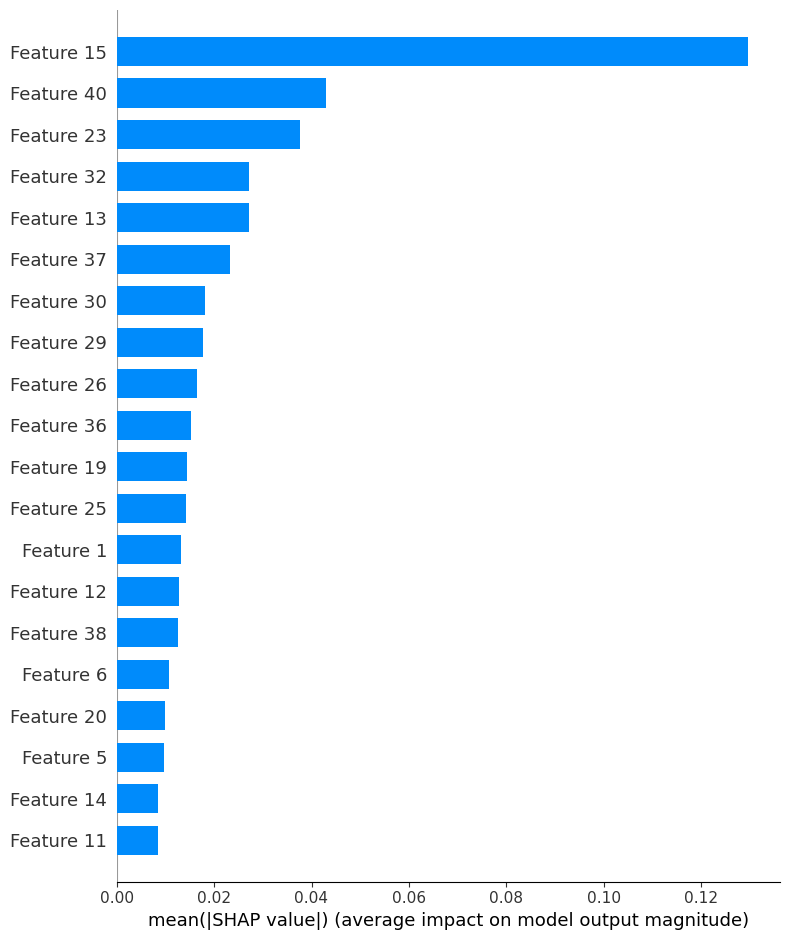
\includegraphics[width=\textwidth]{img/SHAP_RFCTU13_CTU13.png}
\caption{SHAP summary plot for the CTU13 Random Forest model tested against CTU13 data.}\label{fig:shap_rfc_ctu13_ctu13}
\end{figure}

Figure~\ref{fig:shap_rfc_ctu13_ctu13} presents the SHAP summary plot for the Random Forest model trained and tested on CTU13. Features are ranked by importance, with `Bwd Packet Length Mean` and `Flow IAT Min` exerting the greatest influence on predictions. This suggests that packet size in the backward direction (destination to source) and the minimum inter-arrival time between packets are key for detecting botnet traffic in CTU13. This aligns with botnets exhibiting abnormal communication patterns, as discussed in Chapter~\ref{chap:background}, Section~\ref{sec:datasets}.

Other notable features include `Fwd Packet Length Min`, `Fwd Packet Length Max`, and `Fwd IAT Min`, indicating that forward-direction packet characteristics also contribute significantly. The prominence of both spatial (packet size) and temporal (inter-arrival time) features highlights their role in identifying botnet behaviour, consistent with prior research in Chapter~\ref{chap:relevant-work}, Section~\ref{sec:RandomForestIntrusion}.

\subsubsection{Random Forest Model on CICIDS2017}\label{subsec:rf-cicids2017}

\begin{figure}[H]
\centering
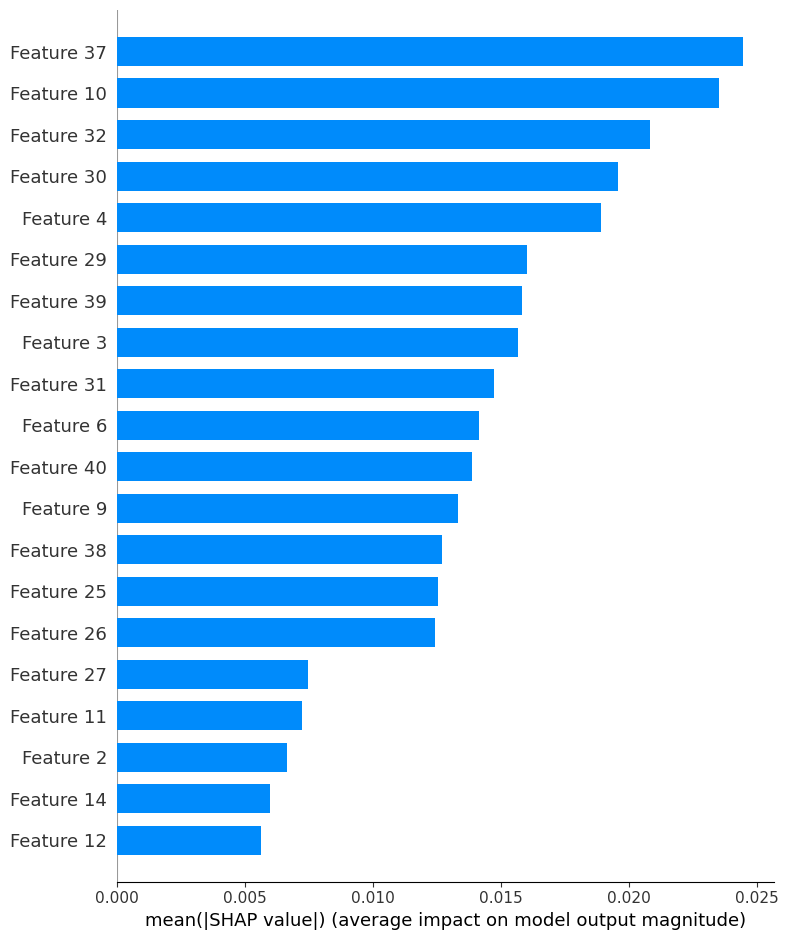
\includegraphics[width=\textwidth]{img/SHAP_RFCICIDS2017_CICIDS2017.png}
\caption{SHAP summary plot for the CICIDS2017 Random Forest model tested against CICIDS2017 data.}\label{fig:shap_rfc_cicids2017_cicids2017}
\end{figure}

For the Random Forest model on CICIDS2017 (Figure~\ref{fig:shap_rfc_cicids2017_cicids2017}), the feature importance differs. `Fwd Packet Length Max` and `Average Packet Size` lead, followed by `Bwd Packet Length Std` and `Flow Duration`. The focus on forward-direction packet sizes underscores their discriminative power for CICIDS2017 attacks, as noted in Chapter~\ref{chap:background}, Section~\ref{sec:datasets}. The high ranking of `Average Packet Size` suggests deviations from typical profiles signal malicious activity, while `Flow Duration` emphasises temporal relevance, aligning with prior analyses in Chapter~\ref{chap:relevant-work}, Section~\ref{sec:RandomForestIntrusion}.

The variation in feature importance between CTU13 and CICIDS2017 highlights dataset-specific discriminative attributes, motivating transferability studies to address RQ1 and RQ3, as outlined in Chapter~\ref{chap:specification-design}, Section~\ref{sec:TransferabilityEvaluation}.

\subsection{Performance on Different Datasets}\label{subsec:performance-different-dataset}

\begin{figure}[H]
\centering
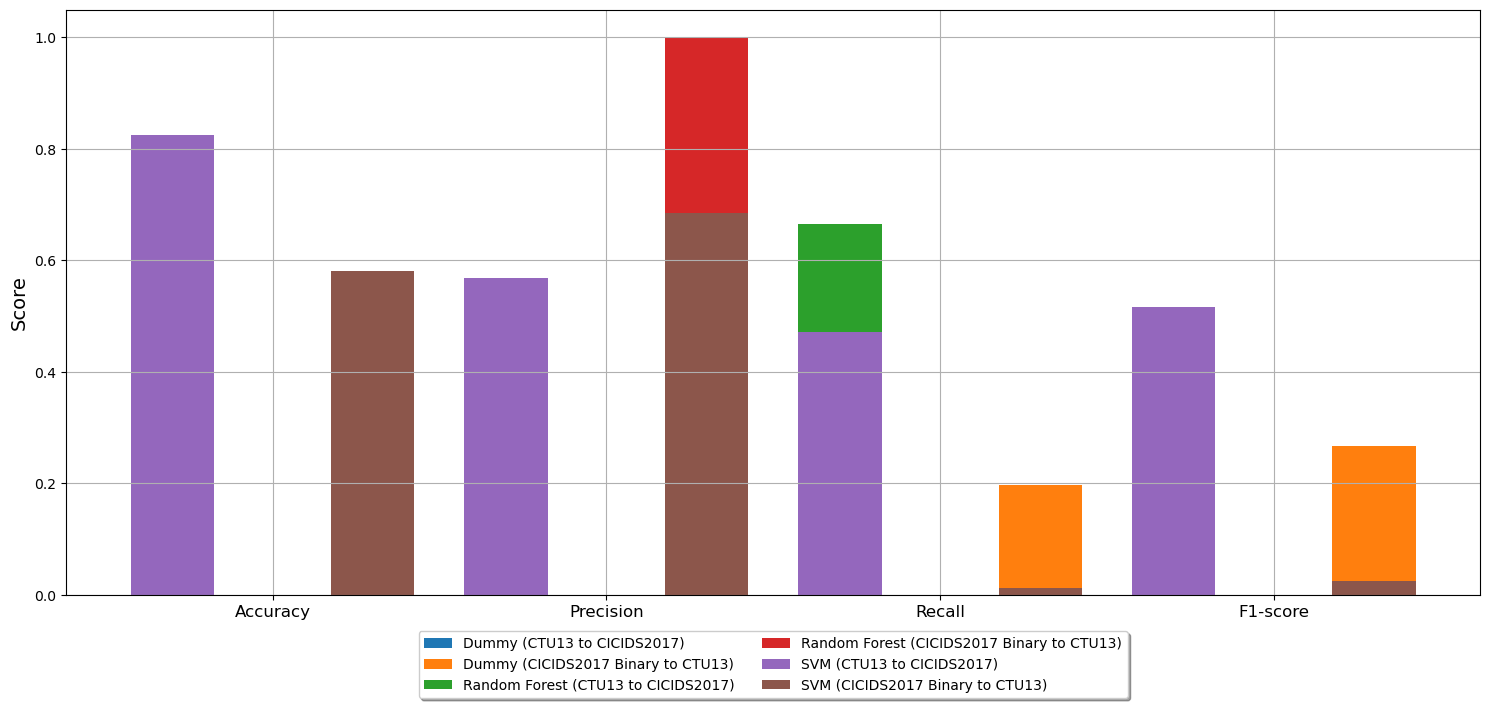
\includegraphics[width=1\textwidth]{img/Classifier_Performance _Across_Datasets.png}
\caption{Classifiers' performance across datasets.}\label{fig:classifier_performance_across_dataset}
\end{figure}

To evaluate transferability, we assessed model performance on datasets different from their training sets, as shown in Figure~\ref{fig:classifier_performance_across_dataset}. The Random Forest model trained on CICIDS2017 and tested on CTU13 exhibited a significant performance drop: accuracy fell to 0.58, precision to 0.65, recall to 0.02, and F1 score to 0.04. This indicates that patterns learned on CICIDS2017 do not translate effectively to CTU13 botnet detection, reflecting challenges in cross-dataset model transfer, as discussed in Chapter~\ref{chap:relevant-work}, Section~\ref{sec:ChallengesLimitations}.

Low recall suggests the model misses much of the botnet traffic in CTU13, possibly due to differing attack profiles or overfitting to CICIDS2017-specific patterns. This underscores dataset bias impacts and the need for representative training data, addressing RQ2, per Chapter~\ref{chap:specification-design}, Section~\ref{sec:TransferabilityEvaluation}.

Conversely, the SVM trained on CTU13 and tested on CICIDS2017 showed improved transferability, with an accuracy of 0.83, precision of 0.57, recall of 0.49, and F1 score of 0.53. Though still below dummy classifier benchmarks, this outperforms its CTU13 baseline, suggesting more transferable decision boundaries than the Random Forest in the reverse direction. However, performance remains suboptimal, with a precision-recall balance indicating many false positives and negatives, reflecting network traffic dynamics and attack evolution challenges, as noted in Chapter~\ref{chap:relevant-work}, Section~\ref{sec:ChallengesLimitations}.

These results highlight cross-dataset performance degradation due to differences in distributions, attack types, and feature profiles. Addressing these requires advanced techniques like transfer learning and domain adaptation, as explored in Chapter~\ref{chap:conclusion-future-work}.

\subsection{Feature Importance Analysis on Different Datasets}\label{subsec:feature-importance-analysis-different-datasets}

We further examined SHAP feature importance for models applied to different datasets, with interpretation guidance in appendix listing~\ref{chap:feature-list}.

\subsubsection{Random Forest Model on CTU13 Tested on CICIDS2017}\label{subsec:rf-ctu13-cicids2017}

\begin{figure}[H]
\centering
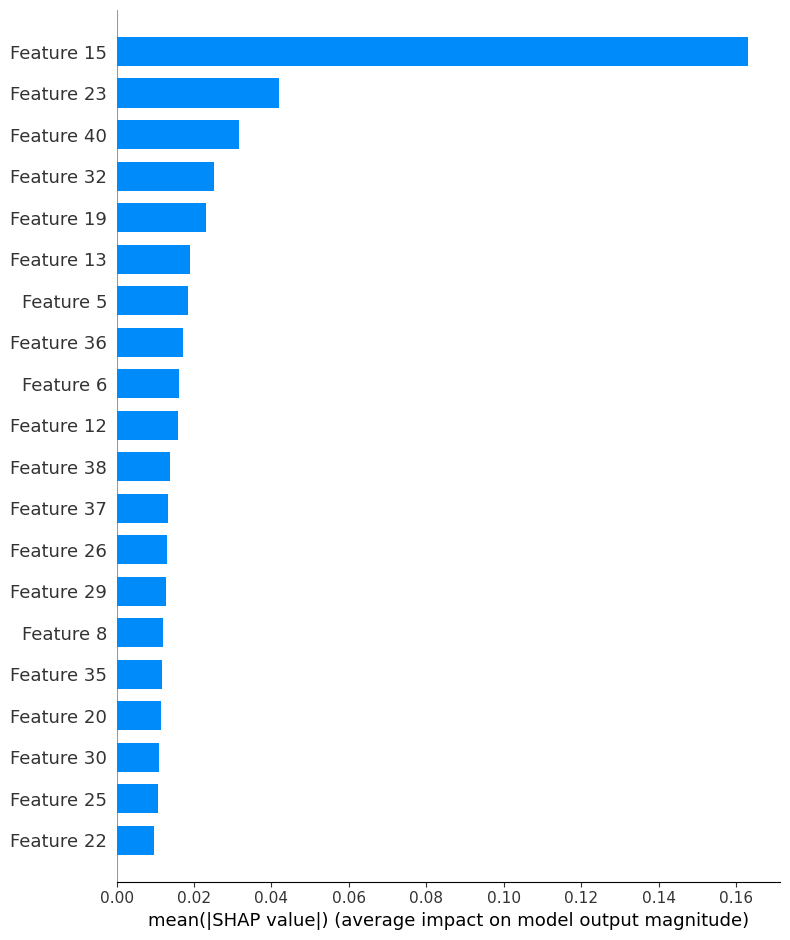
\includegraphics[width=\textwidth]{img/SHAP_RFCTU13_CICIDS2017.png}
\caption{SHAP summary plot for the CTU13 Random Forest model tested against CICIDS2017 data.}\label{fig:shap_rfc_ctu13_cicids2017}
\end{figure}

Figure~\ref{fig:shap_rfc_ctu13_cicids2017} shows SHAP values for the CTU13-trained Random Forest applied to CICIDS2017. Compared to Figure~\ref{fig:shap_rfc_ctu13_ctu13}, feature rankings shift: `Bwd Packet Length Mean` remains key, but `Init Win bytes backward` and `Flow Packets/s` rise in importance. This suggests reliance on different features due to CICIDS2017’s distinct traffic profiles, with `Init Win bytes backward` potentially better distinguishing attack flows.

Despite this shift, the model's classification performance remains suboptimal with data unlike its training set. This highlights transferability challenges, as discussed in Chapter~\ref{chap:conclusion-future-work}.

\subsubsection{Random Forest Model on CICIDS2017 Tested on CTU13}\label{subsec:rf-cicids2017-ctu13}

\begin{figure}[H]
\centering
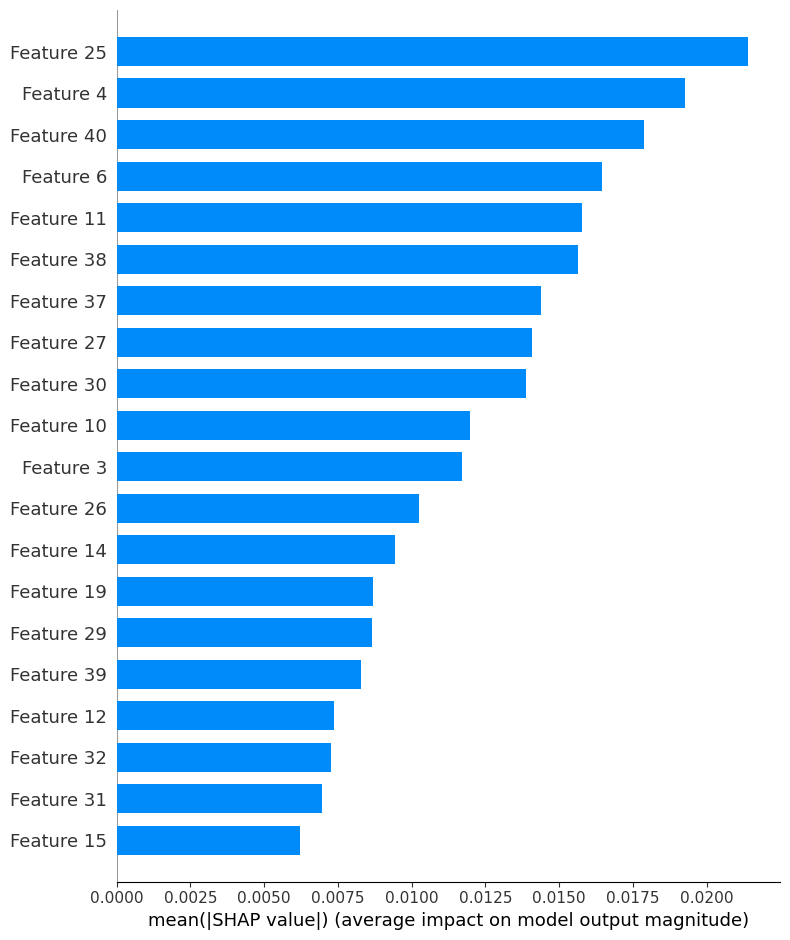
\includegraphics[width=\textwidth]{img/SHAP_RFCICIDS2017_CTU13.png}
\caption{SHAP summary plot for the CICIDS2017 Random Forest model tested against CTU13 data.}\label{fig:shap_rfc_cicids2017_ctu13}
\end{figure}

Figure~\ref{fig:shap_rfc_cicids2017_ctu13} illustrates feature importance for the CICIDS2017-trained Random Forest on CTU13. Compared to Figure~\ref{fig:shap_rfc_cicids2017_cicids2017}, `Bwd Packet Length Std` and `Fwd IAT Total` overtake `Fwd Packet Length Max` and `Average Packet Size`, reflecting a focus on backward packet variation and forward inter-arrival times. However, this aligns with poor performance, reinforcing cross-dataset application difficulties, as noted in Chapter~\ref{chap:relevant-work}, Section~\ref{sec:ChallengesLimitations}.

SHAP analysis across datasets offers insights into pattern transferability and feature relevance for attack detection, addressing RQ3 (Chapter~\ref{chap:specification-design}, Section~\ref{sec:TransferabilityEvaluation}). Feature importance shifts and performance impacts highlight dataset biases and direct application limits, per Chapter~\ref{chap:relevant-work}, Section~\ref{sec:ChallengesLimitations}.

These findings emphasise the need for advanced techniques—transfer learning, domain adaptation, and robust feature engineering—to enhance transferability and generalisation in network intrusion detection models, as discussed in Chapter~\ref{chap:conclusion-future-work}. Developing adaptable, interpretable models can lead to reliable machine learning-based systems for detecting evolving cyber threats across diverse network environments.